\documentclass[11pt]{article}

\usepackage[margin=1in]{geometry}
\usepackage{amsmath,amssymb,amsthm}
\usepackage{booktabs}
\usepackage{enumitem}
\usepackage{hyperref}
\usepackage{xcolor}
\usepackage{tikz}
\usetikzlibrary{arrows.meta,positioning,fit,calc,shapes.geometric}

\title{Lecture~7 Study Notes:\\Attention and Self-Attention}
\author{Deep Learning Notes\\
\small Ground-up intuitions and worked examples\\[0.35em]
\small Formation borrows heavily from the
\href{https://r-three.github.io/deep-learning-lecture-notes/}{CSC2516 course lecture notes}}
\date{}

\begin{document}
\maketitle

\begin{abstract}
These notes develop \textbf{attention} from first principles---with extra
detail, intuition, and simple numerical examples---so the ideas are easier
to follow from the ground up. Attention is introduced as an associative
memory, as a soft one-nearest-neighbor classifier, and as the mechanism that
fixes the information bottleneck in sequence-to-sequence models. The notes
then specialize to \textbf{self-attention} (the core of the transformer),
including path length, a fully worked toy example, position encodings, and
multi-headed attention. A final section shows \textbf{attention pooling}
inside a small end-to-end network that maps a variable-length sequence to a
scalar prediction. Content formation borrows heavily from the original
\href{https://r-three.github.io/deep-learning-lecture-notes/}{CSC2516 course
lecture notes}.
\end{abstract}

\tableofcontents
\vspace{1em}

%----------------------------------------------------------------------
\section{Attention as an Associative Memory}
%----------------------------------------------------------------------

Attention is usefully viewed as the neural-network version of an
\emph{associative memory}, or key--value store. To build one, fix five
ingredients:

\begin{enumerate}[leftmargin=*]
  \item a \textbf{query} --- the identifier of what we want to retrieve;
  \item a set of \textbf{keys} --- identifiers attached to stored items;
  \item a set of \textbf{values} --- one payload per key;
  \item a \textbf{comparison} function that scores the query against each key;
  \item a \textbf{reduction} function that combines the values according to
        those scores.
\end{enumerate}

\noindent\textbf{Definition.}
An attention mechanism is completely specified by these five ingredients.
Comparison produces a vector of scores \(\mathbf{a}\); reduction maps
\(\{\mathbf{v}_1,\ldots,\mathbf{v}_N\}\) and \(\mathbf{a}\) to a single
vector in \(\mathbb{R}^{d_v}\).

\paragraph{Python dictionary (hard attention).}
A dictionary compares by equality (in practice, hashing) and returns the
unique matching value. That assignment is hard and non-differentiable, so
it cannot sit inside a network trained by gradient descent. The rest of
these notes softens the same idea: replace exact match with a continuous
score, and replace hard selection with a weighted average.

\paragraph{Notation.}
Keys \(\mathbf{k}_i\in\mathbb{R}^{d_k}\), query \(\mathbf{q}\in\mathbb{R}^{d_q}\)
(often \(d_q=d_k\)), values \(\mathbf{v}_i\in\mathbb{R}^{d_v}\). Scores
\(a_i=\alpha(\mathbf{q},\mathbf{k}_i)\). Attention acts on a \emph{set}:
shuffling key--value pairs together leaves the result unchanged
(permutation invariance). That property will matter when we apply attention
to sequences.

\noindent\textbf{One-line intuition (kept throughout).}
Comparison chooses \emph{where} to look; reduction copies \emph{what} to
read.

%----------------------------------------------------------------------
\section{A Soft One-Nearest-Neighbor Classifier}
%----------------------------------------------------------------------

A one-nearest-neighbor (1-NN) classifier is rarely introduced as attention,
but it uses the same five ingredients and makes the soft version easy to
see.

\begin{center}
\begin{tabular}{@{}ll@{}}
\toprule
Ingredient & 1-NN reading \\
\midrule
Query  & the test point \(\mathbf{q}\) to classify \\
Keys   & training inputs \(\mathbf{k}_i=\mathbf{x}^{(i)}\) \\
Values & training labels \(v_i=t^{(i)}\) \\
Comparison & negated distance
  \(\alpha(\mathbf{q},\mathbf{k}_i)=-\lVert\mathbf{q}-\mathbf{k}_i\rVert\) \\
Reduction (hard) & \(\operatorname{argmax}(\mathbf{a})\cdot V\)
  (label of the closest point) \\
\bottomrule
\end{tabular}
\end{center}

Negating distance turns ``closest'' into ``largest score,'' so
\(\operatorname{argmax}\) selects the nearest neighbor. Hard
\(\operatorname{argmax}\) has derivative zero almost everywhere, so it is
not usable inside a trained network.

\paragraph{Softening.}
Replace \(\operatorname{argmax}\) by \(\operatorname{softmax}\):
\[
  f(\{\mathbf{v}_1,\ldots,\mathbf{v}_N\},\mathbf{a})
  =
  \operatorname{softmax}(\mathbf{a})\cdot V.
\]
The result is no longer strictly 1-NN: it averages nearby labels in
proportion to closeness. Neural attention mechanisms look like this soft
1-NN, with a different comparison function and with values that need not be
class labels.

\begin{quote}
\emph{Exam / interview note.} Framing 1-NN as attention is a common
conceptual check: the five ingredients, then soft \(\operatorname{argmax}\)
via softmax.
\end{quote}

%----------------------------------------------------------------------
\section{Sequence-to-Sequence with Attention}
%----------------------------------------------------------------------

Attention first became widespread in neural networks inside
\emph{sequence-to-sequence} (seq2seq) models, so we briefly revisit the
encoder--decoder RNN before leaving recurrence behind.

\subsection{The information bottleneck}

Without attention, an encoder RNN consumes the input
\(x_1,\ldots,x_T\) and summarizes it with a single fixed context
\(\mathbf{c}=\mathbf{h}_T\) (the last encoder state). A decoder RNN is
initialized from \(\mathbf{c}\) and emits the output sequence. For long
inputs this is a bottleneck: every relevant detail must be compressed into
one fixed-length vector, and every decoder step must rely on that same
summary---even when the next output word depends on only one source word.

\paragraph{Translation intuition.}
English ``the cat sat on the mat'' \(\to\) French ``le chat s'est assis sur
le tapis.'' Producing \emph{tapis} mainly needs \emph{mat}, not the whole
sentence. A single \(\mathbf{c}=\mathbf{h}_T\) cannot specialize per output
step.

\subsection{Per-step context via attention (Bahdanau et al., 2015)}

Compute a fresh context \(\mathbf{c}_{t'}\) at each decoder step \(t'\),
focused on the source positions relevant to the word about to be written.
Fill in the five ingredients:

\begin{itemize}[leftmargin=*]
  \item \textbf{Query:} previous decoder state \(\mathbf{s}_{t'-1}\)
        (cannot use \(\mathbf{s}_{t'}\), which will depend on
        \(\mathbf{c}_{t'}\));
  \item \textbf{Keys and values:} encoder states
        \(\mathbf{h}_1,\ldots,\mathbf{h}_T\);
  \item \textbf{Comparison:} a small MLP (encoder and decoder live in
        different spaces),
        \[
          a_t
          =
          \mathbf{w}_v^\top
          \tanh\!\bigl(\mathbf{W}_q\mathbf{s}_{t'-1}
          + \mathbf{W}_k\mathbf{h}_t\bigr);
        \]
  \item \textbf{Reduction:} softmax-weighted average
        \[
          \mathbf{c}_{t'}
          =
          \sum_{t=1}^{T}\alpha_t\,\mathbf{h}_t,
          \qquad
          \boldsymbol{\alpha}=\operatorname{softmax}(\mathbf{a}).
        \]
\end{itemize}

The decoder then consumes the context at every step,
\[
  \mathbf{s}_{t'}
  =
  g\bigl(\mathbf{s}_{t'-1},\, y_{t'-1},\, \mathbf{c}_{t'}\bigr),
\]
e.g.\ by concatenating \(\mathbf{c}_{t'}\) with the previous output embedding.
Information about the input is no longer forced through a single vector;
each output step re-selects what to read.

\subsection{Where attention sits in the encoder--decoder}

Figure~\ref{fig:seq2seq-attn} places the attention block between the
encoder states (keys/values) and the decoder (query). Softmax chooses
\emph{where} among \(h_1,\ldots,h_T\) to look; the weighted sum builds the
context that the decoder reads.

\begin{figure}[ht]
\centering
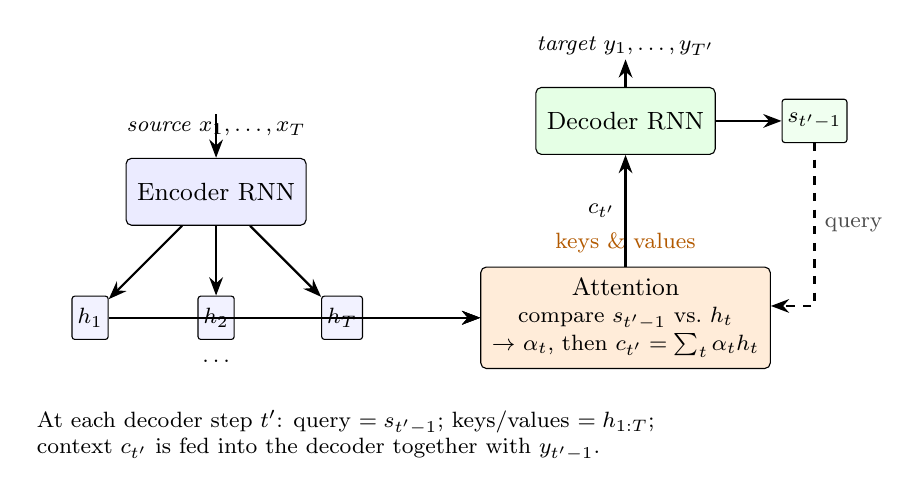
\begin{tikzpicture}[
  font=\small,
  >=Stealth,
  box/.style={draw, rounded corners=2pt, align=center,
              minimum height=0.85cm, inner sep=4pt},
  tinybox/.style={draw, rounded corners=1pt, align=center,
                  minimum height=0.55cm, inner sep=2pt, font=\footnotesize},
  arr/.style={->, thick},
  dashedarr/.style={->, thick, dashed},
]
  % Encoder column
  \node[box, fill=blue!8] (enc) at (0,0)
    {Encoder RNN};
  \node[tinybox, fill=blue!5] (h1) at (-1.6,-1.6) {\(h_1\)};
  \node[tinybox, fill=blue!5] (h2) at (0,-1.6) {\(h_2\)};
  \node[tinybox, fill=blue!5] (hT) at (1.6,-1.6) {\(h_T\)};
  \node[font=\footnotesize] at (0,-2.15) {\(\ldots\)};
  \draw[arr] (enc) -- (h1);
  \draw[arr] (enc) -- (h2);
  \draw[arr] (enc) -- (hT);
  \node[above=0.15cm of enc, font=\footnotesize\itshape]
    {source \(x_1,\ldots,x_T\)};
  \draw[arr] ([yshift=0.55cm]enc.north) -- (enc.north);

  % Attention block
  \node[box, fill=orange!15, minimum width=3.4cm] (attn) at (5.2,-1.6)
    {Attention\\[-1pt]
     {\footnotesize compare \(s_{t'-1}\) vs.\ \(h_t\)}\\[-1pt]
     {\footnotesize \(\to\) \(\alpha_t\), then
      \(c_{t'}=\sum_t\alpha_t h_t\)}};
  \draw[arr] (h1) -- (attn);
  \draw[arr] (h2) -- (attn);
  \draw[arr] (hT) -- (attn);
  \node[above=0.05cm of attn, font=\footnotesize, text=orange!70!black]
    {keys \& values};

  % Decoder column
  \node[box, fill=green!10] (dec) at (5.2,0.9)
    {Decoder RNN};
  \node[font=\footnotesize\itshape] at (5.2,1.85)
    {target \(y_{1},\ldots,y_{T'}\)};
  \draw[arr] (dec.north) -- ++(0,0.35);
  \node[tinybox, fill=green!6] (st) at (7.6,0.9) {\(s_{t'-1}\)};
  \draw[arr] (dec) -- (st);
  \draw[dashedarr] (st.south) |- ([yshift=0.15cm]attn.east)
    node[pos=0.25, right, font=\footnotesize, text=black!70] {query};
  \draw[arr] (attn) -- (dec)
    node[midway, left, font=\footnotesize] {\(c_{t'}\)};

  % Bottom caption inside figure
  \node[font=\footnotesize, align=left, anchor=west] at (-2.4,-3.1) {%
    At each decoder step \(t'\): query \(=s_{t'-1}\);
    keys/values \(=h_{1:T}\);\\
    context \(c_{t'}\) is fed into the decoder together with \(y_{t'-1}\).};
\end{tikzpicture}
\caption{RNN encoder--decoder with attention. The encoder produces states
\(h_1,\ldots,h_T\). At decoder step \(t'\), attention scores the previous
decoder state against every encoder state, softmax-normalizes, and forms
context \(c_{t'}\). Without attention, a single \(c=h_T\) would replace
this whole block.}
\label{fig:seq2seq-attn}
\end{figure}

Clock convention used below: primed index \(t'\) is the \emph{decoder /
output} clock; unprimed \(t\) is the \emph{encoder / source} clock.
Encoder states stay fixed; the attention weights change with \(t'\).

%----------------------------------------------------------------------
\section{Self-Attention Setup}
%----------------------------------------------------------------------

Seq2seq attention works, but the mechanism that dominates modern models is
\textbf{self-attention}: queries, keys, and values all come from the
\emph{same} sequence. The layer still maps a length-\(T\) sequence to a
length-\(T\) sequence (like an RNN layer), but without recurrence.

Start with token vectors \(x_1,x_2,\ldots,x_T\in\mathbb{R}^{m}\) (e.g.\ word
embeddings, or outputs of a previous layer). Project every token with three
learned matrices shared across positions:
\begin{align}
  q_t &= W_Q x_t, \label{eq:q} \\
  k_t &= W_K x_t, \label{eq:k} \\
  v_t &= W_V x_t. \label{eq:v}
\end{align}

\begin{center}
\begin{tabular}{@{}lll@{}}
\toprule
Vector & Role & Intuition \\
\midrule
query \(q_t\)  & ``what am I looking for?''   & search request \\
key \(k_t\)    & ``what do I advertise?''     & index / label \\
value \(v_t\)  & ``what content do I offer?'' & payload to copy \\
\bottomrule
\end{tabular}
\end{center}

\noindent\textbf{Shapes.}
\(W_Q,W_K\in\mathbb{R}^{d_k\times m}\) and \(W_V\in\mathbb{R}^{d_v\times m}\).
Queries and keys share dimension \(d_k\) so a dot product is well-defined.
Values may use a different \(d_v\).

Comparison is a scaled dot product,
\[
  \alpha(q,k_i)=\frac{q^\top k_i}{\sqrt{d_k}},
\]
and reduction is again a softmax-weighted average of the values. Scaling by
\(\sqrt{d_k}\) keeps score variance from growing with dimension (and
prevents a saturated, nearly one-hot softmax that hurts gradients).

After the projections we have three length-\(T\) sequences---queries, keys,
and values---ready to be compared. The next sections walk through every
matrix with tiny numbers; afterward we return to \emph{why} this rewrite
is attractive via path length.

%----------------------------------------------------------------------
\section{Baby Toy Example: The Ingredients}
%----------------------------------------------------------------------

We use deliberately tiny dimensions so every matrix can be written out.

\subsection{Inputs}

Sequence length \(T=3\), embedding size \(m=2\):
\[
  x_1 = \begin{bmatrix}1\\0\end{bmatrix},\quad
  x_2 = \begin{bmatrix}0\\1\end{bmatrix},\quad
  x_3 = \begin{bmatrix}1\\1\end{bmatrix}.
\]
Think of these as embeddings of three tokens, e.g.\ ``the'', ``cat'', ``sat''.
Stacked as a matrix \(X \in \mathbb{R}^{T \times m}\):
\[
  X =
  \begin{bmatrix}
    1 & 0 \\
    0 & 1 \\
    1 & 1
  \end{bmatrix}.
\]

\subsection{Weight matrices}

Choose \(d_k = d_v = 2\). Pick simple numbers (in a real model these are learned):
\[
  W_Q = \begin{bmatrix}1&0\\0&1\end{bmatrix},\quad
  W_K = \begin{bmatrix}1&1\\0&1\end{bmatrix},\quad
  W_V = \begin{bmatrix}1&0\\1&1\end{bmatrix}.
\]
All three are \(2\times 2\) because \(m=d_k=d_v=2\).

\subsection{Queries, keys, and values}

For one token, e.g.\ \(x_1\):
\begin{align*}
  q_1 &= W_Q x_1 = \begin{bmatrix}1&0\\0&1\end{bmatrix}\begin{bmatrix}1\\0\end{bmatrix}
       = \begin{bmatrix}1\\0\end{bmatrix}, \\
  k_1 &= W_K x_1 = \begin{bmatrix}1&1\\0&1\end{bmatrix}\begin{bmatrix}1\\0\end{bmatrix}
       = \begin{bmatrix}1\\0\end{bmatrix}, \\
  v_1 &= W_V x_1 = \begin{bmatrix}1&0\\1&1\end{bmatrix}\begin{bmatrix}1\\0\end{bmatrix}
       = \begin{bmatrix}1\\1\end{bmatrix}.
\end{align*}
Doing this for every token:

\begin{center}
\begin{tabular}{@{}cccc@{}}
\toprule
token & \(q_t\) & \(k_t\) & \(v_t\) \\
\midrule
\(x_1\) & \(\begin{bmatrix}1\\0\end{bmatrix}\)
        & \(\begin{bmatrix}1\\0\end{bmatrix}\)
        & \(\begin{bmatrix}1\\1\end{bmatrix}\) \\[1.2em]
\(x_2\) & \(\begin{bmatrix}0\\1\end{bmatrix}\)
        & \(\begin{bmatrix}1\\1\end{bmatrix}\)
        & \(\begin{bmatrix}0\\1\end{bmatrix}\) \\[1.2em]
\(x_3\) & \(\begin{bmatrix}1\\1\end{bmatrix}\)
        & \(\begin{bmatrix}2\\1\end{bmatrix}\)
        & \(\begin{bmatrix}1\\2\end{bmatrix}\) \\
\bottomrule
\end{tabular}
\end{center}

\noindent\textbf{Where do \(v_1,v_2,v_3\) come from?}
Each is just \(v_t = W_V x_t\). Same idea as queries and keys, different matrix.
The big value matrix \(V\) is those vectors stacked as rows:
\[
  V =
  \begin{bmatrix}
    \text{---}\, v_1^\top\, \text{---} \\
    \text{---}\, v_2^\top\, \text{---} \\
    \text{---}\, v_3^\top\, \text{---}
  \end{bmatrix}
  =
  \begin{bmatrix}
    1 & 1 \\
    0 & 1 \\
    1 & 2
  \end{bmatrix}
  \in \mathbb{R}^{T \times d_v}
  = \mathbb{R}^{3\times 2}.
\]
Analogously one can form \(Q\) and \(K\) by stacking the \(q_t^\top\) and
\(k_t^\top\) as rows.

%----------------------------------------------------------------------
\section{Step 1: Scaled Attention Scores}
%----------------------------------------------------------------------

For each query, score every key with a \textbf{scaled} dot product:
\[
  s_{tj}
  =
  \frac{q_t^\top k_j}{\sqrt{d_k}}.
\]
Here \(d_k=2\), so \(\sqrt{d_k}=\sqrt{2}\approx 1.414\).

\paragraph{Token 1 (\(q_1\)).}
\begin{align*}
  q_1^\top k_1 &= 1 &\Rightarrow\quad s_{11} &= \tfrac{1}{\sqrt{2}} \approx 0.707, \\
  q_1^\top k_2 &= 1 &\Rightarrow\quad s_{12} &= \tfrac{1}{\sqrt{2}} \approx 0.707, \\
  q_1^\top k_3 &= 2 &\Rightarrow\quad s_{13} &= \tfrac{2}{\sqrt{2}} = \sqrt{2} \approx 1.414.
\end{align*}

\paragraph{Token 2 (\(q_2\)).}
\begin{align*}
  q_2^\top k_1 &= 0 &\Rightarrow\quad s_{21} = 0, \\
  q_2^\top k_2 &= 1 &\Rightarrow\quad s_{22} = \tfrac{1}{\sqrt{2}} \approx 0.707, \\
  q_2^\top k_3 &= 1 &\Rightarrow\quad s_{23} = \tfrac{1}{\sqrt{2}} \approx 0.707.
\end{align*}

\paragraph{Token 3 (\(q_3\)).}
\begin{align*}
  q_3^\top k_1 &= 1 &\Rightarrow\quad s_{31} = \tfrac{1}{\sqrt{2}} \approx 0.707, \\
  q_3^\top k_2 &= 2 &\Rightarrow\quad s_{32} = \sqrt{2} \approx 1.414, \\
  q_3^\top k_3 &= 3 &\Rightarrow\quad s_{33} = \tfrac{3}{\sqrt{2}} \approx 2.121.
\end{align*}

Scaled score matrix (row \(t\) = scores for query \(t\)):
\[
  S
  =
  \frac{QK^\top}{\sqrt{d_k}}
  \approx
  \begin{bmatrix}
    0.707 & 0.707 & 1.414 \\
    0.000 & 0.707 & 0.707 \\
    0.707 & 1.414 & 2.121
  \end{bmatrix}.
\]
Shape: \(T\times T\). Every token looks at every token.

\noindent\textbf{Why divide by \(\sqrt{d_k}\)?}
Raw dot products grow with dimension. Scaling keeps the values fed into
softmax from becoming extremely large, which would make the attention
weights too peaked (nearly one-hot) and hard to train.

%----------------------------------------------------------------------
\section{Step 2: Softmax --- ``Where Should I Look?''}
%----------------------------------------------------------------------

Turn each row of \(S\) into weights that sum to \(1\):
\[
  A_{tj}
  =
  \frac{\exp(s_{tj})}{\sum_{j'=1}^{T}\exp(s_{tj'})}.
\]

\begin{align*}
  \alpha_1 &= \mathrm{softmax}([0.707,\,0.707,\,1.414])
           \approx [0.248,\,0.248,\,0.503], \\
  \alpha_2 &= \mathrm{softmax}([0.000,\,0.707,\,0.707])
           \approx [0.198,\,0.401,\,0.401], \\
  \alpha_3 &= \mathrm{softmax}([0.707,\,1.414,\,2.121])
           \approx [0.140,\,0.284,\,0.576].
\end{align*}

Attention weight matrix:
\[
  A \approx
  \begin{bmatrix}
    0.248 & 0.248 & 0.503 \\
    0.198 & 0.401 & 0.401 \\
    0.140 & 0.284 & 0.576
  \end{bmatrix}.
\]
Each row sums to \(1\). Entry \(A_{tj}\) means:
\emph{how much does token \(t\) listen to token \(j\)?}

Softmax alone only gives a ranking / allocation of attention.
It does not yet move any content.

%----------------------------------------------------------------------
\section{Step 3: Weighted Sum of Values --- ``What Should I Read?''}
%----------------------------------------------------------------------

This is the \textbf{retrieval} step:
\[
  y_t = \sum_{j=1}^{T} A_{tj}\, v_j
  \qquad\text{or, in matrix form,}\qquad
  Y = AV.
\]

\subsection{Intuition}

\begin{itemize}[leftmargin=*]
  \item \(A\) answers \emph{where} to look (percentages).
  \item \(V\) holds the \emph{content} you might copy (after \(W_V\)).
  \item \(y_t = \sum_j A_{tj} v_j\) builds a new vector as a blend of
        everyone's values, with more weight on the tokens that matched
        the query strongly.
\end{itemize}

Without multiplying by \(V\), attention would only give you a ranking.
With it, you get a new representation that actually contains information
from the useful tokens.

\paragraph{Concrete reading of token 1.}
Weights \(\alpha_1 \approx [0.25,\,0.25,\,0.50]\) say:
``listen a little to token~1, a little to token~2, and about half to token~3.''
Then
\[
  y_1 \approx 0.25\,v_1 + 0.25\,v_2 + 0.50\,v_3
\]
is mostly like \(v_3\), with some \(v_1\) and \(v_2\) mixed in.
Token~1's new vector is rewritten using content from the tokens its query matched.

\paragraph{Why this matters.}
\begin{enumerate}[leftmargin=*]
  \item \textbf{Context injection.}
        A bare embedding of ``it'' is vague. After this step, ``it'' can absorb
        value-features from ``cat'' if its query matched the key of ``cat''.
  \item \textbf{Soft lookup.}
        Hard selection would pick one token only. Softmax + weighted sum lets
        you grab a main token and keep a bit of others, and gradients flow
        through all of them.
  \item \textbf{Same length, richer meaning.}
        You keep \(T\) outputs, but each is no longer ``just me''; it is
        ``me, plus the parts of the sequence I needed.''
\end{enumerate}

\subsection{Numbers for the toy}

\begin{align*}
  y_1 &\approx 0.248\,v_1 + 0.248\,v_2 + 0.503\,v_3
       \approx \begin{bmatrix}0.752\\1.503\end{bmatrix}, \\
  y_2 &\approx 0.198\,v_1 + 0.401\,v_2 + 0.401\,v_3
       \approx \begin{bmatrix}0.599\\1.401\end{bmatrix}, \\
  y_3 &\approx 0.140\,v_1 + 0.284\,v_2 + 0.576\,v_3
       \approx \begin{bmatrix}0.716\\1.576\end{bmatrix}.
\end{align*}

Output matrix:
\[
  Y \approx
  \begin{bmatrix}
    0.752 & 1.503 \\
    0.599 & 1.401 \\
    0.716 & 1.576
  \end{bmatrix}.
\]

%----------------------------------------------------------------------
\section{Putting It Together: Length \(T\) In \(\to\) Length \(T\) Out}
%----------------------------------------------------------------------

\begin{center}
\begin{tabular}{@{}lll@{}}
\toprule
Stage & Object & Shape \\
\midrule
input     & \(x_1,x_2,x_3\) & \(T=3\) vectors of size \(m=2\) \\
project   & \(Q,K,V\) & still \(T\) vectors each \\
scores    & \(S = QK^\top / \sqrt{d_k}\) & \(T\times T\) \\
weights   & \(A = \mathrm{softmax}(S)\) & \(T\times T\) \\
output    & \(y_1,y_2,y_3 = AV\) & \(T=3\) vectors of size \(d_v=2\) \\
\bottomrule
\end{tabular}
\end{center}

The full self-attention formula is
\[
  \boxed{
    Y
    =
    \mathrm{Attention}(Q,K,V)
    =
    \mathrm{softmax}\!\left(\frac{QK^\top}{\sqrt{d_k}}\right)V.
  }
\]
You never collapse the sequence. Each position keeps its own output; that
output is a soft mix of all values, with mix weights chosen by that
position's query:
\[
  \underbrace{(x_1,\ldots,x_T)}_{T\ \text{inputs}}
  \;\xrightarrow{\;W_Q,W_K,W_V\;}\;
  (Q,K,V)
  \;\xrightarrow{\;\mathrm{softmax}(QK^\top/\sqrt{d_k})\,V\;}\;
  \underbrace{(y_1,\ldots,y_T)}_{T\ \text{outputs}}.
\]

\noindent\textbf{Self-attention vs.\ encoder--decoder attention.}
In the encoder--decoder case, the query came from the decoder and the
states being averaged came from the encoder. In self-attention, one
sequence supplies \(Q\), \(K\), and \(V\), so each token can gather
context from the rest of the \emph{same} sentence (including itself).

%----------------------------------------------------------------------
\section{Position Encoding: Why Self-Attention Needs Order}
%----------------------------------------------------------------------

Self-attention alone is \textbf{orderless}. Attention treats keys and values
as a \emph{set}: shuffling the inputs shuffles the outputs the same way
(permutation equivariance). That is fine for a bag of items, but bad for
language --- ``the cat sat'' does not mean the same as ``sat the cat.''
To process sequences we must inject position into either the inputs or the
comparison scores.

\begin{center}
\begin{tabular}{@{}clp{7.2cm}@{}}
\toprule
\# & Method & What it does \\
\midrule
0 & Absolute embeddings (early)
  & Add a learned vector \(e_t\) to input \(x_t\) \\
(i) & Relative key shift
  & Add a learned vector \(\mathbf{p}_{ij}\) to the key \\
(ii) & Relative bias
  & Add a learned scalar \(p_{ij}\) to the score \\
(iii) & RoPE
  & Rotate \(q_i\) and \(k_j\) by angles depending on \(i,j\) \\
\bottomrule
\end{tabular}
\end{center}

Relative methods depend on the \textbf{offset} \(i-j\) (up to some maximum),
so they extrapolate past training lengths better than absolute embeddings.

\subsection{Shared baby setup}

Two tokens, dimension \(d_k=2\). For clarity we sometimes omit
\(\sqrt{d_k}\) (the story is unchanged with scaling):
\[
  q_1=\begin{bmatrix}1\\0\end{bmatrix},\;
  q_2=\begin{bmatrix}0\\1\end{bmatrix},\qquad
  k_1=\begin{bmatrix}1\\0\end{bmatrix},\;
  k_2=\begin{bmatrix}0\\1\end{bmatrix}.
\]
Without position info, scores are just \(q_i^\top k_j\):
\[
  S
  =
  \begin{bmatrix}
    q_1^\top k_1 & q_1^\top k_2 \\
    q_2^\top k_1 & q_2^\top k_2
  \end{bmatrix}
  =
  \begin{bmatrix}
    1 & 0 \\
    0 & 1
  \end{bmatrix}.
\]
If we swap the two tokens, this pattern just swaps with them. Order is not
truly ``seen''; only content matching is.

%----------------------------------------------------------------------
\subsection{Absolute position embeddings (early approach)}
%----------------------------------------------------------------------

Learn a vector \(e_t\) for each index and \textbf{add it before} projecting:
\[
  \tilde{x}_t = x_t + e_t,
  \qquad
  q_t = W_Q \tilde{x}_t,\;\ldots
\]

\paragraph{Baby example.}
Let
\[
  e_1=\begin{bmatrix}1\\0\end{bmatrix},\qquad
  e_2=\begin{bmatrix}0\\1\end{bmatrix}.
\]
Suppose two tokens have the \emph{same content}
\(x_1=x_2=\begin{bmatrix}0\\0\end{bmatrix}\)
(so without PE they are identical). After adding positions,
\[
  \tilde{x}_1=e_1,\qquad \tilde{x}_2=e_2.
\]
They are no longer the same, so \(q_1\neq q_2\) and \(k_1\neq k_2\).
Softmax can treat ``token at position~1'' differently from ``token at
position~2'' even if the words were identical.

\paragraph{Order preserved?}
Yes: if a word moves from slot~1 to slot~2, it picks up \(e_2\) instead of
\(e_1\), so scores change.

\paragraph{Weakness.}
Embeddings are only learned up to the longest training length \(T_{\max}\).
A longer test sequence has no \(e_{T_{\max}+1}\). This absolute approach is
uncommon today for that reason.

%----------------------------------------------------------------------
\subsection{Method (i): Relative vector on the key}
%----------------------------------------------------------------------

Idea: leave the query alone; \textbf{add a learned position vector to the
key} before the dot product. The vector depends only on the offset
\(i-j\):
\[
  \alpha(q_i,k_j)
  =
  \frac{q_i^\top (k_j + \mathbf{p}_{ij})}{\sqrt{d_k}},
  \qquad
  \mathbf{p}_{ij} = \mathbf{p}_{i-j}.
\]

\paragraph{Initial vectors (content only).}
Reuse the shared baby \(q\) and \(k\):
\[
  q_1=\begin{bmatrix}1\\0\end{bmatrix},\;
  q_2=\begin{bmatrix}0\\1\end{bmatrix},\qquad
  k_1=\begin{bmatrix}1\\0\end{bmatrix},\;
  k_2=\begin{bmatrix}0\\1\end{bmatrix}.
\]
Content-only scores (no position yet):
\[
  S_{\text{content}}
  =
  \begin{bmatrix}
    q_1^\top k_1 & q_1^\top k_2 \\
    q_2^\top k_1 & q_2^\top k_2
  \end{bmatrix}
  =
  \begin{bmatrix}1&0\\0&1\end{bmatrix}.
\]

\paragraph{Position table we will add.}
One learned vector per offset (for \(T=2\)):
\[
  \mathbf{p}_{0}=\begin{bmatrix}0\\0\end{bmatrix},\quad
  \mathbf{p}_{+1}=\begin{bmatrix}1\\0\end{bmatrix},\quad
  \mathbf{p}_{-1}=\begin{bmatrix}0\\1\end{bmatrix}.
\]

\paragraph{Step-by-step: inject position into each key, then score.}
For every pair \((i,j)\):
\begin{enumerate}[leftmargin=*]
  \item Start with the content key \(k_j\).
  \item Look up the offset \(i-j\) and fetch \(\mathbf{p}_{i-j}\).
  \item Form the position-aware key
        \(\tilde{k}_{ij} := k_j + \mathbf{p}_{i-j}\).
  \item Score: \(s_{ij} = q_i^\top \tilde{k}_{ij}\)
        (optionally divide by \(\sqrt{d_k}\)).
\end{enumerate}

\textbf{Pair \((1,1)\)} --- offset \(0\):
\begin{align*}
  k_1 &= \begin{bmatrix}1\\0\end{bmatrix}, \\
  \tilde{k}_{11}
    &= k_1 + \mathbf{p}_{0}
     = \begin{bmatrix}1\\0\end{bmatrix}+\begin{bmatrix}0\\0\end{bmatrix}
     = \begin{bmatrix}1\\0\end{bmatrix}, \\
  s_{11}
    &= q_1^\top \tilde{k}_{11}
     = \begin{bmatrix}1&0\end{bmatrix}\begin{bmatrix}1\\0\end{bmatrix}
     = 1.
\end{align*}

\textbf{Pair \((1,2)\)} --- offset \(1-2=-1\):
\begin{align*}
  k_2 &= \begin{bmatrix}0\\1\end{bmatrix}, \\
  \tilde{k}_{12}
    &= k_2 + \mathbf{p}_{-1}
     = \begin{bmatrix}0\\1\end{bmatrix}+\begin{bmatrix}0\\1\end{bmatrix}
     = \begin{bmatrix}0\\2\end{bmatrix}, \\
  s_{12}
    &= q_1^\top \tilde{k}_{12}
     = \begin{bmatrix}1&0\end{bmatrix}\begin{bmatrix}0\\2\end{bmatrix}
     = 0.
\end{align*}

\textbf{Pair \((2,1)\)} --- offset \(+1\):
\begin{align*}
  k_1 &= \begin{bmatrix}1\\0\end{bmatrix}, \\
  \tilde{k}_{21}
    &= k_1 + \mathbf{p}_{+1}
     = \begin{bmatrix}1\\0\end{bmatrix}+\begin{bmatrix}1\\0\end{bmatrix}
     = \begin{bmatrix}2\\0\end{bmatrix}, \\
  s_{21}
    &= q_2^\top \tilde{k}_{21}
     = \begin{bmatrix}0&1\end{bmatrix}\begin{bmatrix}2\\0\end{bmatrix}
     = 0.
\end{align*}

\textbf{Pair \((2,2)\)} --- offset \(0\):
\begin{align*}
  \tilde{k}_{22}
    &= k_2 + \mathbf{p}_{0}
     = \begin{bmatrix}0\\1\end{bmatrix}, \\
  s_{22}
    &= q_2^\top \tilde{k}_{22}
     = 1.
\end{align*}

\paragraph{What you end with.}
Position-aware score matrix:
\[
  S_{(i)}
  =
  \begin{bmatrix}1&0\\0&1\end{bmatrix}
  =
  S_{\text{content}}
  \quad\text{(with this particular \(\mathbf{p}\) table)}.
\]
The \emph{keys that were actually used} are no longer the raw \(k_j\); they
are the position-shifted versions
\[
  \tilde{k}_{11}=\begin{bmatrix}1\\0\end{bmatrix},\;
  \tilde{k}_{12}=\begin{bmatrix}0\\2\end{bmatrix},\;
  \tilde{k}_{21}=\begin{bmatrix}2\\0\end{bmatrix},\;
  \tilde{k}_{22}=\begin{bmatrix}0\\1\end{bmatrix}.
\]
If we change \(\mathbf{p}_{+1}\) to \(\begin{bmatrix}2\\0\end{bmatrix}\),
then \(s_{21}=q_2^\top\begin{bmatrix}3\\0\end{bmatrix}=0\) still here, but
a query with a nonzero first component would get a boost when looking
\emph{backward}. Different offsets use different \(\mathbf{p}\), so
``A then B'' and ``B then A'' can produce different scores even when A and
B have similar content.

\paragraph{Cost.}
One learned vector of size \(d_k\) per offset --- somewhat costly.

%----------------------------------------------------------------------
\subsection{Method (ii): Relative scalar bias}
%----------------------------------------------------------------------

Idea: keep the content key unchanged; \textbf{add a learned scalar to the
score} after the content dot product. The scalar depends only on the offset
\(i-j\):
\[
  \alpha(q_i,k_j)
  =
  \frac{q_i^\top k_j}{\sqrt{d_k}} + p_{ij},
  \qquad
  p_{ij}=p_{i-j}.
\]

\paragraph{Initial vectors (content only).}
Same baby \(q\) and \(k\) as above. Content-only score matrix:
\[
  S_{\text{content}}
  =
  \begin{bmatrix}
    q_1^\top k_1 & q_1^\top k_2 \\
    q_2^\top k_1 & q_2^\top k_2
  \end{bmatrix}
  =
  \begin{bmatrix}1&0\\0&1\end{bmatrix}.
\]
Notice: here we do \emph{not} modify \(k_j\) itself. The vectors
\(q_i\) and \(k_j\) stay exactly as they are.

\paragraph{Position table we will add.}
One learned scalar per offset (``prefer attending to the previous token''):
\[
  p_{0}=0,\qquad p_{+1}=+2,\qquad p_{-1}=-1.
\]

\paragraph{Step-by-step: compute content score, then add the bias.}
For every pair \((i,j)\):
\begin{enumerate}[leftmargin=*]
  \item Start with content vectors \(q_i\) and \(k_j\) (unchanged).
  \item Content score: \(s^{\text{content}}_{ij}=q_i^\top k_j\).
  \item Look up offset \(i-j\) and fetch scalar \(p_{i-j}\).
  \item Position-aware score:
        \(s_{ij}=s^{\text{content}}_{ij}+p_{i-j}\).
\end{enumerate}

\textbf{Pair \((1,1)\)} --- offset \(0\):
\[
  s^{\text{content}}_{11}=1,\quad
  p_{0}=0,\quad
  s_{11}=1+0=1.
\]

\textbf{Pair \((1,2)\)} --- offset \(-1\):
\[
  s^{\text{content}}_{12}=0,\quad
  p_{-1}=-1,\quad
  s_{12}=0+(-1)=-1.
\]

\textbf{Pair \((2,1)\)} --- offset \(+1\):
\[
  s^{\text{content}}_{21}=0,\quad
  p_{+1}=+2,\quad
  s_{21}=0+2=2.
\]

\textbf{Pair \((2,2)\)} --- offset \(0\):
\[
  s^{\text{content}}_{22}=1,\quad
  p_{0}=0,\quad
  s_{22}=1+0=1.
\]

\paragraph{What you end with.}
\[
  S_{(ii)}
  =
  S_{\text{content}}
  +
  \underbrace{\begin{bmatrix}
    p_{0} & p_{-1} \\
    p_{+1} & p_{0}
  \end{bmatrix}}_{\text{position bias matrix}}
  =
  \begin{bmatrix}1&0\\0&1\end{bmatrix}
  +
  \begin{bmatrix}0&-1\\2&0\end{bmatrix}
  =
  \begin{bmatrix}1&-1\\2&1\end{bmatrix}.
\]
Softmax on row~2 (scores \([2,1]\)) puts more weight on position~1 --- the
previous token --- than on itself. That preference is \emph{purely
positional}; the content vectors never changed.

If you swap the sequence, the bias table is still indexed by positions
\((i,j)\), so the favored ``previous'' neighbor is a different word. Order
matters. Cheaper than~(i): one number per offset, not a \(d_k\)-vector.

%----------------------------------------------------------------------
\subsection{Method (iii): RoPE (rotary position encoding)}
%----------------------------------------------------------------------

Idea: do not add a table of \(p\)'s. Instead, \textbf{rotate} the query by
an angle depending on its absolute index \(i\), and rotate the key by an
angle depending on \(j\). Relative position appears automatically in the
dot product:
\[
  \alpha(q_i,k_j)
  =
  \frac{(R_i q_i)^\top (R_j k_j)}{\sqrt{d_k}}.
\]
In 2D, rotation by \(\phi\) is
\[
  R(\phi)
  =
  \begin{bmatrix}
    \cos\phi & -\sin\phi \\
    \sin\phi & \cos\phi
  \end{bmatrix}.
\]
\textbf{Key identity:}
\[
  (R_i q)^\top (R_j k)
  =
  q^\top R_i^\top R_j k
  =
  q^\top R_{j-i}\, k.
\]
So the score depends on the relative angle \((j-i)\theta\).

\paragraph{Initial vectors (content only).}
Take a single content direction for a clear demo:
\[
  q=\begin{bmatrix}1\\0\end{bmatrix},\qquad
  k=\begin{bmatrix}1\\0\end{bmatrix}.
\]
Without RoPE, \(q^\top k=1\) no matter where they sit. Position has not
entered yet.

\paragraph{Position rotations we will apply.}
Fix \(\theta=\pi/2\) (90°). Absolute rotations for indices \(0,1,2\):
\begin{align*}
  R_0 &= R(0)
       = \begin{bmatrix}1&0\\0&1\end{bmatrix}
       \quad\text{(identity; no rotation)}, \\
  R_1 &= R(\pi/2)
       = \begin{bmatrix}0&-1\\1&0\end{bmatrix}, \\
  R_2 &= R(\pi)
       = \begin{bmatrix}-1&0\\0&-1\end{bmatrix}.
\end{align*}

\paragraph{Step-by-step: rotate each vector by its absolute position.}
For a query at index \(i\) and a key at index \(j\):
\begin{enumerate}[leftmargin=*]
  \item Start with content vectors \(q\) and \(k\).
  \item Form the position-aware query
        \(\tilde{q}_i := R_i q\).
  \item Form the position-aware key
        \(\tilde{k}_j := R_j k\).
  \item Score: \(s_{ij}=\tilde{q}_i^\top \tilde{k}_j\)
        (equivalently \(q^\top R_{j-i}\,k\)).
\end{enumerate}

\textbf{Case A --- same position} (\(i=j=0\), offset \(0\)):
\begin{align*}
  \tilde{q}_0 &= R_0 q = \begin{bmatrix}1\\0\end{bmatrix}, \\
  \tilde{k}_0 &= R_0 k = \begin{bmatrix}1\\0\end{bmatrix}, \\
  s_{00}
    &= \tilde{q}_0^\top \tilde{k}_0
     = 1.
\end{align*}
Initial \(q,k\) are unchanged because \(R_0=I\).

\textbf{Case B --- key one step ahead} (\(i=0\), \(j=1\), offset \(+1\)):
\begin{align*}
  \tilde{q}_0 &= R_0 q = \begin{bmatrix}1\\0\end{bmatrix}
  \quad\text{(query still ``pointing right'')}, \\
  \tilde{k}_1 &= R_1 k
               = \begin{bmatrix}0&-1\\1&0\end{bmatrix}
                 \begin{bmatrix}1\\0\end{bmatrix}
               = \begin{bmatrix}0\\1\end{bmatrix}
  \quad\text{(key now ``pointing up'')}, \\
  s_{01}
    &= \tilde{q}_0^\top \tilde{k}_1
     = \begin{bmatrix}1&0\end{bmatrix}\begin{bmatrix}0\\1\end{bmatrix}
     = 0.
\end{align*}

\textbf{Case C --- query at 1, key at 2} (still offset \(+1\)):
\begin{align*}
  \tilde{q}_1 &= R_1 q = \begin{bmatrix}0\\1\end{bmatrix}, \\
  \tilde{k}_2 &= R_2 k = \begin{bmatrix}-1\\0\end{bmatrix}, \\
  s_{12}
    &= \tilde{q}_1^\top \tilde{k}_2
     = \begin{bmatrix}0&1\end{bmatrix}\begin{bmatrix}-1\\0\end{bmatrix}
     = 0.
\end{align*}
Same relative offset as Case~B \(\Rightarrow\) same score \(0\), even though
absolute indices differ. That is the relative property of RoPE.

\paragraph{What you end with.}
\begin{center}
\begin{tabular}{@{}cccc@{}}
\toprule
Case & Initial \(q,k\) & After rotation & Score \\
\midrule
\(i=j=0\)
  & \(\begin{bmatrix}1\\0\end{bmatrix},\begin{bmatrix}1\\0\end{bmatrix}\)
  & \(\begin{bmatrix}1\\0\end{bmatrix},\begin{bmatrix}1\\0\end{bmatrix}\)
  & \(1\) \\[1.1em]
\(i=0,j=1\)
  & same content
  & \(\begin{bmatrix}1\\0\end{bmatrix},\begin{bmatrix}0\\1\end{bmatrix}\)
  & \(0\) \\[1.1em]
\(i=1,j=2\)
  & same content
  & \(\begin{bmatrix}0\\1\end{bmatrix},\begin{bmatrix}-1\\0\end{bmatrix}\)
  & \(0\) \\
\bottomrule
\end{tabular}
\end{center}
Same content, different offset \(\Rightarrow\) different score. Relative
position is baked into the geometry of the rotated vectors. RoPE needs no
learned \(p\) and is common in modern LLMs.

%----------------------------------------------------------------------
\subsection{How position encoding preserves sequence order}
%----------------------------------------------------------------------

We close by tying the three methods back to the original problem: making
self-attention care about order. Below we start from the \emph{same}
initial content vectors in two different orders and show that, once
position is injected, the final attention scores (and therefore \(Y\))
differ.

\paragraph{Initial content vectors (no position yet).}
Two tokens with contents \(A\) and \(B\):
\[
  x_A=\begin{bmatrix}1\\0\end{bmatrix},\qquad
  x_B=\begin{bmatrix}0\\1\end{bmatrix}.
\]
For a transparent demo, take \(W_Q=W_K=I\), so
\(q=k=x\) at each position, and use method~(ii) biases
\(p_0=0\), \(p_{+1}=+2\), \(p_{-1}=-1\).

\paragraph{Order 1: \(A\) then \(B\) (positions \(1,2\)).}
\begin{enumerate}[leftmargin=*]
  \item Place contents into slots:
        \(x_1=x_A=\begin{bmatrix}1\\0\end{bmatrix}\),
        \(x_2=x_B=\begin{bmatrix}0\\1\end{bmatrix}\).
  \item Content scores:
        \[
          S_{\text{content}}
          =
          \begin{bmatrix}
            x_A^\top x_A & x_A^\top x_B \\
            x_B^\top x_A & x_B^\top x_B
          \end{bmatrix}
          =
          \begin{bmatrix}1&0\\0&1\end{bmatrix}.
        \]
  \item Add position biases by offset:
        \[
          S^{(A,B)}
          =
          \begin{bmatrix}1&0\\0&1\end{bmatrix}
          +
          \begin{bmatrix}0&-1\\2&0\end{bmatrix}
          =
          \begin{bmatrix}1&-1\\2&1\end{bmatrix}.
        \]
  \item Softmax (approx.): row~2 \(\mathrm{softmax}([2,1])\approx[0.73,\,0.27]\).
        So token \(B\) (position~2) pulls \emph{mostly from \(A\)}
        (the previous token).
\end{enumerate}

\paragraph{Order 2: \(B\) then \(A\) (positions \(1,2\)).}
\begin{enumerate}[leftmargin=*]
  \item Same contents, swapped slots:
        \(x_1=x_B=\begin{bmatrix}0\\1\end{bmatrix}\),
        \(x_2=x_A=\begin{bmatrix}1\\0\end{bmatrix}\).
  \item Content scores:
        \[
          S_{\text{content}}
          =
          \begin{bmatrix}
            x_B^\top x_B & x_B^\top x_A \\
            x_A^\top x_B & x_A^\top x_A
          \end{bmatrix}
          =
          \begin{bmatrix}1&0\\0&1\end{bmatrix}.
        \]
        (Same matrix shape of \(1\)s on the diagonal --- content matching
        alone still cannot tell the two orders apart.)
  \item Add the \emph{same} position-bias table (indexed by slots, not by
        word identity):
        \[
          S^{(B,A)}
          =
          \begin{bmatrix}1&0\\0&1\end{bmatrix}
          +
          \begin{bmatrix}0&-1\\2&0\end{bmatrix}
          =
          \begin{bmatrix}1&-1\\2&1\end{bmatrix}.
        \]
  \item Softmax again puts row~2 weight mostly on position~1 --- but
        position~1 is now \(B\), so token \(A\) pulls mostly from \(B\).
\end{enumerate}

\paragraph{What changed?}
\begin{center}
\begin{tabular}{@{}lll@{}}
\toprule
 & Order \(A,B\) & Order \(B,A\) \\
\midrule
Initial slot~1 vector
  & \(x_A=\begin{bmatrix}1\\0\end{bmatrix}\)
  & \(x_B=\begin{bmatrix}0\\1\end{bmatrix}\) \\[0.9em]
Initial slot~2 vector
  & \(x_B=\begin{bmatrix}0\\1\end{bmatrix}\)
  & \(x_A=\begin{bmatrix}1\\0\end{bmatrix}\) \\[0.9em]
After adding position
  & biases favor ``look left''
  & same biases, different neighbor \\
Who does slot~2 read?
  & mostly \(A\)
  & mostly \(B\) \\
\bottomrule
\end{tabular}
\end{center}
Same words, different order \(\Rightarrow\) different mixes in \(Y=AV\).
Without the position step, both orders would produce equivalent
(shuffled) attention; with it, order is preserved.

\paragraph{Without PE vs.\ with PE (summary).}
\begin{itemize}[leftmargin=*]
  \item \textbf{Without PE:} content alone decides scores; shuffling tokens
        shuffles outputs the same way; ``cat sat'' and ``sat cat'' induce
        the same set of interactions.
  \item \textbf{With PE:} position changes vectors (\(x_t+e_t\), rotated
        \(q,k\)) or scores (\(+\,p_{ij}\)); \(A_{ij}\) depends on both
        content match \emph{and} offset/order; softmax still picks where to
        look and values supply what to read, but ``where'' is
        position-aware.
\end{itemize}

\paragraph{One-line map of the three lecture variants.}
\begin{itemize}[leftmargin=*]
  \item \textbf{(i)} Start with \(k_j\); add learned relative vector
        \(\mathbf{p}_{i-j}\); then \(q_i^\top(k_j+\mathbf{p}_{i-j})\).
  \item \textbf{(ii)} Start with \(q_i^\top k_j\); add learned relative
        scalar \(p_{i-j}\) before softmax.
  \item \textbf{(iii)} Start with \(q_i,k_j\); rotate to
        \(R_i q_i\) and \(R_j k_j\); their angle difference carries the
        offset (RoPE).
\end{itemize}
Absolute embeddings add ``I am at index \(t\)'' to the token itself;
relative methods encode ``you are \(i-j\) steps away from me'' inside the
comparison.

%----------------------------------------------------------------------
\section{Why Self-Attention? Path Length}
%----------------------------------------------------------------------

Having seen self-attention compute a length-\(T\) rewrite of its input,
a natural question is why this is attractive compared with convolution or
recurrence. Path length measures how many sequential operations are needed to mix
information between two positions of the input---closely related to the
idea of a receptive field. Consider a length-5 sequence and ask when an
output can depend on both \(x_1\) and \(x_5\).

\begin{center}
\begin{tabular}{@{}lll@{}}
\toprule
Layer & Path length (\(x_1\leftrightarrow x_5\)) & Parallelism \\
\midrule
1D conv (kernel \(3\))
  & \(2\) (receptive field grows by \(2\) per layer)
  & Positions in one layer are parallel; depth is sequential \\
RNN
  & \(5\) (signal travels step by step)
  & Inherently sequential along time \\
Self-attention
  & \(1\) (every output mixes all inputs in one layer)
  & All outputs computable in parallel \\
\bottomrule
\end{tabular}
\end{center}

More generally, for length \(T\): convolution has path length
\(O(T/k)\) for kernel size \(k\); recurrence has path length \(O(T)\);
self-attention has path length \(O(1)\). Short paths are not a guarantee
that optimization will discover long-range dependencies, but they remove
an architectural obstruction: information need not pass through a long
chain of Jacobians.

Path length also counts work that cannot be parallelized. Convolutional
layers stack depth-wise; RNNs wait on the previous time step.
Self-attention outputs are independent weighted averages of the same
inputs, so the layer is a pair of large matrix multiplies---well matched
to modern hardware:
\[
  S=\frac{QK^\top}{\sqrt{d_k}},
  \qquad
  Y=\operatorname{softmax}_{\text{row}}(S)\,V.
\]

%----------------------------------------------------------------------
\section{Multi-Headed Self-Attention}
%----------------------------------------------------------------------

In a transformer we do not run self-attention once. We run \(H\)
\textbf{heads} in parallel --- each an independent self-attention with its
own weights --- then aggregate them. This is analogous to multiple channels
in a CNN: same input, different filters, then combine.

\subsection{Intuition: what a head is (and is not)}

A \textbf{head} is one full self-attention pathway: one triple of weight
matrices
\[
  \bigl(\mathbf{W}_Q^{(i)},\,\mathbf{W}_K^{(i)},\,\mathbf{W}_V^{(i)}\bigr)
\]
plus the scores, softmax weights, and outputs those weights induce on the
shared input \(\mathbf{x}\).

\paragraph{Structurally, every head is the same kind of object.}
Same shapes, same formulas, same steps (project \(\to\) score \(\to\)
softmax \(\to\) weighted values). There is \emph{no} built-in specialty
--- nothing in the definition says ``head~1 does syntax'' or ``head~2
looks at coordinate~1.'' The big \(W\)'s are peers: different
\emph{copies} of the same type of parameters.

\paragraph{What multi-head actually buys you.}
Multi-head means: keep \(H\) separate sets of \(W\)'s. That gives the
model extra capacity --- \(H\) chances to learn \(H\) attention patterns
in parallel --- then \(\mathbf{W}_O\) blends them. Whether those patterns
actually become usefully different is up to training (random init + the
loss). If two heads ended up with identical \(W\)'s, they would compute
identical \(\mathbf{h}^{(i)}\) and the extras would buy nothing.

\paragraph{Why more than one copy can help.}
One triple \((\mathbf{W}_Q,\mathbf{W}_K,\mathbf{W}_V)\) implements only
\emph{one} soft ``who matches whom'' rule. Sequences often need several
rules at once. Multiple parameter copies give room for that; they do not
hard-code what each rule is.

\noindent\textbf{One-line intuition.}
Multi-heads \(=\) different sets of the big \(W\)'s (same architecture,
separate parameters). They offer different opportunities for attention
patterns; there is no inherent structural difference among the \(W\)'s
themselves.

\subsection{Definition (same notation)}

Multi-headed self-attention applies \(H\) independent self-attentions, each
with its own \(\mathbf{W}_Q^{(i)},\mathbf{W}_K^{(i)},\mathbf{W}_V^{(i)}\),
and aggregates with a learned output matrix \(\mathbf{W}_O\).

For each head \(i=1,\ldots,H\),
\[
  \mathbf{h}^{(i)}
  =
  \operatorname{self\text{-}attention}\!\bigl(
  \mathbf{W}_Q^{(i)},\,
  \mathbf{W}_K^{(i)},\,
  \mathbf{W}_V^{(i)},\,
  \mathbf{x}
  \bigr).
\]
Each \(\mathbf{h}^{(i)}\) is a length-\(T\) sequence of vectors in
\(\mathbb{R}^{d_v}\). Stack the \(H\) head outputs at a position and mix:
\[
  \text{Output}
  =
  \mathbf{W}_O
  \begin{bmatrix}
    \mathbf{h}^{(1)} \\[0.25em]
    \mathbf{h}^{(2)} \\[0.25em]
    \vdots \\[0.25em]
    \mathbf{h}^{(H)}
  \end{bmatrix},
  \qquad
  \mathbf{W}_O \in \mathbb{R}^{d_v \times H d_v}.
\]
\(\mathbf{W}_O\) maps the stacked \(H d_v\)-vector back to \(d_v\), so the
layer still emits \(d_v\)-dimensional vectors --- now informed by all heads.

\paragraph{Flow.}
\[
  \mathbf{x}
  \;\longrightarrow\;
  \begin{cases}
  \text{head }1:\;
  \mathbf{W}_Q^{(1)},\mathbf{W}_K^{(1)},\mathbf{W}_V^{(1)}
  \;\to\;\mathbf{h}^{(1)} \\[0.2em]
  \text{head }2:\;
  \mathbf{W}_Q^{(2)},\mathbf{W}_K^{(2)},\mathbf{W}_V^{(2)}
  \;\to\;\mathbf{h}^{(2)} \\[0.2em]
  \vdots \\[0.2em]
  \text{head }H:\;
  \mathbf{W}_Q^{(H)},\mathbf{W}_K^{(H)},\mathbf{W}_V^{(H)}
  \;\to\;\mathbf{h}^{(H)}
  \end{cases}
  \;\xrightarrow{\;\text{stack}\;}
  \mathbb{R}^{H d_v}
  \;\xrightarrow{\;\mathbf{W}_O\;}
  \mathbb{R}^{d_v}.
\]

\subsection{Baby example: setup}

Take \(T=2\), \(H=2\), embedding size \(m=2\), and \(d_k=d_v=1\) so every
projection is a single number (easy to see by hand).

\paragraph{Initial input vectors.}
\[
  \mathbf{x}_1=\begin{bmatrix}1\\0\end{bmatrix},\qquad
  \mathbf{x}_2=\begin{bmatrix}0\\1\end{bmatrix}.
\]
Each \(\mathbf{x}_t\) is just a length-2 list of numbers (two entries).

\paragraph{Head~1 weights} (a teaching choice, not a definition of ``head''):
\[
  \mathbf{W}_Q^{(1)}=\begin{bmatrix}1&0\end{bmatrix},\quad
  \mathbf{W}_K^{(1)}=\begin{bmatrix}1&0\end{bmatrix},\quad
  \mathbf{W}_V^{(1)}=\begin{bmatrix}1&0\end{bmatrix}.
\]

\paragraph{Head~2 weights} (another teaching choice --- different copy of \(W\)):
\[
  \mathbf{W}_Q^{(2)}=\begin{bmatrix}0&1\end{bmatrix},\quad
  \mathbf{W}_K^{(2)}=\begin{bmatrix}0&1\end{bmatrix},\quad
  \mathbf{W}_V^{(2)}=\begin{bmatrix}0&1\end{bmatrix}.
\]

\paragraph{Why these particular numbers?}
Only to make the arithmetic show two heads disagreeing. With
\(\mathbf{W}^{(1)}=\begin{bmatrix}1&0\end{bmatrix}\), each projection
keeps only the \emph{top} entry of \(\mathbf{x}_t\) (feature dim
\(2\to 1\)); sequence length stays \(T=2\). With
\(\mathbf{W}^{(2)}=\begin{bmatrix}0&1\end{bmatrix}\), each projection
keeps only the \emph{bottom} entry. That is a hand-picked illustration
that \textbf{different \(W\)'s \(\Rightarrow\) different \(q,k,v\) and
different \(A\)}. It is \emph{not} claiming that real heads are ``the
first-entry head'' and ``the second-entry head.'' In a trained model each
\(\mathbf{W}^{(i)}\) is a full learned map over all features.

\subsection{Step A --- Head 1 does ordinary self-attention}

\paragraph{1. Project (initial \(\mathbf{x}\) \(\to\) \(q,k,v\)).}
\begin{align*}
  q_1^{(1)} &= \mathbf{W}_Q^{(1)}\mathbf{x}_1
             = \begin{bmatrix}1&0\end{bmatrix}\begin{bmatrix}1\\0\end{bmatrix}
             = 1, \\
  k_1^{(1)} &= \mathbf{W}_K^{(1)}\mathbf{x}_1 = 1, \\
  v_1^{(1)} &= \mathbf{W}_V^{(1)}\mathbf{x}_1 = 1, \\[0.4em]
  q_2^{(1)} &= \mathbf{W}_Q^{(1)}\mathbf{x}_2
             = \begin{bmatrix}1&0\end{bmatrix}\begin{bmatrix}0\\1\end{bmatrix}
             = 0, \\
  k_2^{(1)} &= 0, \\
  v_2^{(1)} &= 0.
\end{align*}

\paragraph{2. Score.}
Since \(d_k=1\), \(\sqrt{d_k}=1\), so
\[
  S^{(1)}
  =
  \begin{bmatrix}
    q_1^{(1)} k_1^{(1)} & q_1^{(1)} k_2^{(1)} \\[0.25em]
    q_2^{(1)} k_1^{(1)} & q_2^{(1)} k_2^{(1)}
  \end{bmatrix}
  =
  \begin{bmatrix}
    1 & 0 \\
    0 & 0
  \end{bmatrix}.
\]

\paragraph{3. Softmax (where to look).}
\[
  A^{(1)}
  =
  \mathrm{row\text{-}softmax}(S^{(1)})
  \approx
  \begin{bmatrix}
    0.73 & 0.27 \\
    0.50 & 0.50
  \end{bmatrix}.
\]
(Row~1 favors position~1; row~2 is uniform because both scores were 0.)

\paragraph{4. Reduce (what to read).}
\[
\begin{aligned}
  h_1^{(1)}
  &=
  0.73\,v_1^{(1)}+0.27\,v_2^{(1)}
  =
  0.73\cdot 1 + 0.27\cdot 0
  \approx 0.73, \\
  h_2^{(1)}
  &=
  0.50\cdot 1 + 0.50\cdot 0
  = 0.50.
\end{aligned}
\]
Head~1 output sequence:
\[
  \mathbf{h}^{(1)} \approx \bigl(0.73,\; 0.50\bigr).
\]

\paragraph{Intuition.}
Same procedure as ordinary self-attention. Because we \emph{chose}
\(\mathbf{W}^{(1)}=\begin{bmatrix}1&0\end{bmatrix}\), the values happen
to be \((v_1^{(1)},v_2^{(1)})=(1,0)\). Softmax on row~1 pulls mostly from
\(v_1^{(1)}\), so \(h_1^{(1)}\) is large; position~2 averages, so
\(h_2^{(1)}\) is mid-sized. The important point is not ``first entry'';
it is that this particular copy of the \(W\)'s induced this particular
\(A^{(1)}\) and \(\mathbf{h}^{(1)}\).

\subsection{Step B --- Head 2, same \(\mathbf{x}\), different weights}

\paragraph{1. Project.}
\begin{align*}
  q_1^{(2)} &= \mathbf{W}_Q^{(2)}\mathbf{x}_1
             = \begin{bmatrix}0&1\end{bmatrix}\begin{bmatrix}1\\0\end{bmatrix}
             = 0, \\
  k_1^{(2)} &= 0,\qquad v_1^{(2)}=0, \\[0.3em]
  q_2^{(2)} &= \mathbf{W}_Q^{(2)}\mathbf{x}_2
             = \begin{bmatrix}0&1\end{bmatrix}\begin{bmatrix}0\\1\end{bmatrix}
             = 1, \\
  k_2^{(2)} &= 1,\qquad v_2^{(2)}=1.
\end{align*}

\paragraph{2--4. Score, softmax, reduce.}
\[
  S^{(2)}
  =
  \begin{bmatrix}
    0 & 0 \\
    0 & 1
  \end{bmatrix},
  \qquad
  A^{(2)}
  \approx
  \begin{bmatrix}
    0.50 & 0.50 \\
    0.27 & 0.73
  \end{bmatrix}.
\]
\[
\begin{aligned}
  h_1^{(2)}
  &= 0.50\cdot 0 + 0.50\cdot 1 = 0.50, \\
  h_2^{(2)}
  &= 0.27\cdot 0 + 0.73\cdot 1 \approx 0.73.
\end{aligned}
\]
Head~2 output sequence:
\[
  \mathbf{h}^{(2)} \approx \bigl(0.50,\; 0.73\bigr).
\]

\paragraph{Intuition.}
Step~B is the \emph{same recipe} as Step~A; the only change is a
\emph{different} set of \(W\)'s. With our toy \(\mathbf{W}^{(2)}\), the
values happen to be \((0,1)\) and the attention pattern flips relative
to head~1:
\[
  A^{(1)}\approx\begin{bmatrix}0.73&0.27\\0.50&0.50\end{bmatrix},
  \qquad
  A^{(2)}\approx\begin{bmatrix}0.50&0.50\\0.27&0.73\end{bmatrix}.
\]
Same \(\mathbf{x}\); different parameter copies \(\Rightarrow\) different
\(A\) and \(\mathbf{h}\). If instead \(\mathbf{W}^{(2)}=\mathbf{W}^{(1)}\),
Steps~A and~B would be identical --- there is no magic that forces heads
apart beyond having separate parameters that training may (or may not)
differentiate.

\subsection{Step C --- Stack heads and mix with \(\mathbf{W}_O\)}

At each position \(t\), stack the two head outputs. Here each head output
is a scalar (\(d_v=1\)), so the stack is 2-dimensional:
\[
  \begin{bmatrix}
    h_t^{(1)} \\[0.25em]
    h_t^{(2)}
  \end{bmatrix}
  \in \mathbb{R}^{H d_v} = \mathbb{R}^{2}.
\]
Lecture shape: \(\mathbf{W}_O \in \mathbb{R}^{d_v \times H d_v}
= \mathbb{R}^{1\times 2}\). Pick a simple mixer that sums the two heads:
\[
  \mathbf{W}_O = \begin{bmatrix}1 & 1\end{bmatrix}.
\]

\paragraph{Position 1 --- initial stacked vector, then mix.}
\begin{align*}
  \begin{bmatrix} h_1^{(1)} \\ h_1^{(2)} \end{bmatrix}
  &\approx
  \begin{bmatrix} 0.73 \\ 0.50 \end{bmatrix}, \\[0.3em]
  \text{output}_1
  &=
  \mathbf{W}_O
  \begin{bmatrix} h_1^{(1)} \\ h_1^{(2)} \end{bmatrix}
  \approx
  \begin{bmatrix}1&1\end{bmatrix}
  \begin{bmatrix}0.73\\0.50\end{bmatrix}
  = 1.23.
\end{align*}

\paragraph{Position 2.}
\begin{align*}
  \begin{bmatrix} h_2^{(1)} \\ h_2^{(2)} \end{bmatrix}
  &\approx
  \begin{bmatrix} 0.50 \\ 0.73 \end{bmatrix}, \\[0.3em]
  \text{output}_2
  &\approx
  \begin{bmatrix}1&1\end{bmatrix}
  \begin{bmatrix}0.50\\0.73\end{bmatrix}
  = 1.23.
\end{align*}

\paragraph{What you end with.}
A length-\(T=2\) sequence of \(d_v\)-dimensional outputs
\[
  \bigl(\text{output}_1,\;\text{output}_2\bigr)
  \approx
  \bigl(1.23,\; 1.23\bigr),
\]
each built from \emph{both} heads.

\paragraph{Intuition for \(\mathbf{W}_O\).}
\begin{itemize}[leftmargin=*]
  \item \(\mathbf{W}_O=\begin{bmatrix}1&0\end{bmatrix}\):
        keep head~1 only; ignore head~2.
  \item \(\mathbf{W}_O=\begin{bmatrix}0&1\end{bmatrix}\):
        keep head~2 only.
  \item \(\mathbf{W}_O=\begin{bmatrix}0.5&0.5\end{bmatrix}\):
        average the two views.
  \item \(\mathbf{W}_O=\begin{bmatrix}1&1\end{bmatrix}\) (our choice):
        sum / amplify both.
\end{itemize}
In a real network \(\mathbf{W}_O\) is learned, so gradient descent decides
how to blend the \(H\) head outputs (whatever patterns their separate
\(W\)'s happened to learn) into one vector per position.

\subsection{Single-head vs.\ multi-head}

\begin{center}
\begin{tabular}{@{}lll@{}}
\toprule
 & Single-head & Multi-head \\
\midrule
Input
  & \(\mathbf{x}_1,\ldots,\mathbf{x}_T\)
  & same \\
Weights
  & one \(\mathbf{W}_Q,\mathbf{W}_K,\mathbf{W}_V\)
  & \(H\) copies of the same kind of \(W\)'s \\
Structure of each head
  & ---
  & identical architecture; only parameters differ \\
Attention
  & one matrix \(A\)
  & \(H\) matrices \(A^{(i)}\) (may or may not differ) \\
Before mix
  & \(d_v\)
  & \(H d_v\) (stacked) \\
Final size
  & \(d_v\)
  & still \(d_v\), via \(\mathbf{W}_O\) \\
Length
  & \(T\to T\)
  & \(T\to T\) \\
\bottomrule
\end{tabular}
\end{center}

\subsection{Summary of the baby walk-through}

\begin{enumerate}[leftmargin=*]
  \item \textbf{Start:}
        \(\mathbf{x}_1=\begin{bmatrix}1\\0\end{bmatrix}\),
        \(\mathbf{x}_2=\begin{bmatrix}0\\1\end{bmatrix}\).
  \item \textbf{Head~1:} project with \(\mathbf{W}^{(1)}\) \(\to\)
        scores \(S^{(1)}\) \(\to\) weights \(A^{(1)}\) \(\to\)
        \(\mathbf{h}^{(1)}\approx(0.73,\,0.50)\).
  \item \textbf{Head~2:} same \(\mathbf{x}\), different \(\mathbf{W}^{(2)}\)
        \(\to\) \(\mathbf{h}^{(2)}\approx(0.50,\,0.73)\).
  \item \textbf{Stack} at each \(t\):
        \(\begin{bmatrix}h_t^{(1)}\\h_t^{(2)}\end{bmatrix}\).
  \item \textbf{Mix:} \(\text{output}_t=\mathbf{W}_O[\cdots]\); still
        length \(T\), dimension \(d_v\).
\end{enumerate}

\noindent\textbf{Remember:}
\emph{a head = one copy of \((\mathbf{W}_Q,\mathbf{W}_K,\mathbf{W}_V)\)
running ordinary self-attention. Multi-head = \(H\) such copies (same
structure, separate parameters), stacked and blended by \(\mathbf{W}_O\).
No inherent role is baked into any head.}

%----------------------------------------------------------------------
\section{Attention Pooling in a Full Network}
%----------------------------------------------------------------------

Self-attention rewrites a length-\(T\) sequence into another length-\(T\)
sequence. A closely related pattern---\textbf{attention pooling}---collapses
a variable-length sequence into \emph{one} context vector, then feeds that
vector to a small feed-forward head. The five attention ingredients are
unchanged; only the query source and output shape differ.

\subsection{Pooling vs.\ self-attention}

\begin{center}
\begin{tabular}{@{}llp{5.2cm}@{}}
\toprule
 & Attention pooling & Self-attention \\
\midrule
Query
  & \textbf{One} learned \(q\) (or \(H\) queries for multi-head)
  & One \(q_t=W_Q x_t\) \textbf{per position} \\
Keys / values
  & Feature vectors \(h_t\) (often after a dense layer); often \(v_t=h_t\)
  & \(k_t=W_K x_t\), \(v_t=W_V x_t\) \\
Output length
  & \textbf{One} context \(c\) per sequence
  & \textbf{\(T\)} outputs \(y_1,\ldots,y_T\) \\
Typical role
  & Summarize sequence \(\to\) predict a scalar / class
  & Rewrite each token with context \\
\bottomrule
\end{tabular}
\end{center}

Same core reduction \(c=\sum_t\alpha_t v_t\) with
\(\alpha=\mathrm{softmax}(e)\); different query source and output shape.

\subsection{Demonstrated example: selective marked sum}

As a concrete end-to-end illustration, consider sequences whose tokens are
2D vectors \((\text{value},\,\text{mark})\):

\begin{center}
\begin{tabular}{@{}lcccccc@{}}
\toprule
 & Pos~0 & Pos~1 & Pos~2 & Pos~3 & \ldots & later \\
\midrule
value & \(0.5\) & \(-0.7\) & \(\mathbf{0.3}\) & \(0.1\) & \ldots & \(\mathbf{0.9}\) \\
mark  & \(0\) & \(0\) & \(\mathbf{1}\) & \(0\) & \ldots & \(\mathbf{1}\) \\
\bottomrule
\end{tabular}
\end{center}

\begin{itemize}[leftmargin=*]
  \item \textbf{Input \(X\):} the whole sequence of these vectors.
  \item \textbf{Target \(y\):} sum of values where mark \(=1\)
        (here \(y=0.3+0.9=1.2\)).
  \item \textbf{Prediction \(\hat{y}\):} the network's scalar output.
  \item \textbf{Loss:} \(\mathrm{MSE}(\hat{y},\,y)\).
\end{itemize}

Attention receives no separate supervision. The regression loss alone
trains every parameter---including the query and any scoring weights---so
that \(\alpha_t\) learns to focus on marked positions. Construction of
layers creates parameters; the forward pass applies them to a batch to
produce \(\hat{y}\); training repeats forward \(\to\) loss \(\to\)
backward \(\to\) optimizer step.

\subsection{Where attention sits in the network}

\[
\begin{aligned}
X &\in \mathbb{R}^{B\times T\times 2}
  &&\text{(batch of sequences)} \\
h &= \mathrm{Dense}_1(X)
  &&\in \mathbb{R}^{B\times T\times d}
  \quad\text{(position-wise)} \\
c &= \mathrm{AttnPool}(h;\,q)
  &&\in \mathbb{R}^{B\times d}
  \quad\text{(one vector per example)} \\
\hat{y} &= \mathrm{Out}(\mathrm{Dense}_2(c))
  &&\in \mathbb{R}^{B\times 1}
  \quad\text{(predicted marked sum)}.
\end{aligned}
\]

Keys and values are typically both \(h\). Softmax chooses \emph{where} to
look; \(h_t\) supplies \emph{what} to average. This is the same reduction
seen in seq2seq attention, but with a \emph{learned} query instead of a
decoder state, and with a scalar head instead of a next-token RNN.

\subsection{Score functions (pooling form)}

One shared query \(q\) for the whole sequence:
\begin{align*}
\text{Bahdanau (additive):} &\quad
  e_t = q^\top \tanh(W_a h_t + b_a), \\
\text{Scaled dot-product:} &\quad
  e_t = \frac{q^\top h_t}{\sqrt{d}}, \\
\text{Multiplicative:} &\quad
  e_t = q^\top W_a h_t
  \quad\text{(no \(\tanh\), no bias)}.
\end{align*}
Then \(\alpha=\mathrm{softmax}(e)\) and \(c=\sum_t \alpha_t h_t\).

\paragraph{Multi-head pooling.}
Use \(H\) queries \(q^{(1)},\ldots,q^{(H)}\) on the same keys/values,
obtain \(H\) contexts, concatenate, and mix with a learned \(W_O\) back to
model dimension. Same idea as multi-headed self-attention: separate
parameter copies, no built-in specialty per head; the output is still one
pooled vector per sequence.

\subsection{Padding and attention masks}

Sequences in a batch may differ in length. Padding to a common
\(T_{\max}\) requires a mask so padded positions do not enter the softmax:
\[
  \texttt{attention\_mask}[b,t]
  =
  \begin{cases}
  1 & \text{if position \(t\) is padding}, \\
  0 & \text{if it is a real token}.
  \end{cases}
\]
Before softmax, set \(e_t=-\infty\) on pads so \(\alpha_t\approx 0\).
Without masking, padding steals attention mass and corrupts \(c\).

\subsection{Training loop in brief}

\paragraph{One training step.}
Load \((X,y,\mathrm{mask})\); forward \(\hat{y}=f_\theta(X,\mathrm{mask})\);
compute \(\ell=\mathrm{MSE}(\hat{y},y)\); backpropagate (gradients reach
dense layers \emph{and} attention parameters); optimizer step (often with
gradient clipping).

\paragraph{Validation / prediction.}
Same forward without gradient tracking: no parameter updates. Validation
tracks generalization; prediction collects \(\hat{y}\) (e.g.\ against \(y\)
on a scatter plot) to check that the network recovers marked sums.

\subsection{Pseudocode overview}

\begin{verbatim}
# ----- Data -----
for each example:
    X = [(v_t, m_t)] for t = 1..T     # m_t in {0,1}
    y = sum of v_t where m_t == 1     # regression target

# ----- Batching -----
pad sequences in a batch to length T_max
mask[b,t] = 1 if pad else 0

# ----- Model forward -----
h = Dense1(X)                         # (B, T, d), position-wise
e_t = score(q, h_t)                   # Bahdanau / dot / multiplicative
e_t = -inf if mask_t else e_t
alpha = softmax(e) over t
c = sum_t alpha_t * h_t               # pooled context (B, d)
y_hat = Out(Dense2(c))                # (B, 1)

# ----- Train step -----
loss = MSE(y_hat, y)
loss.backward()
optimizer.step()
\end{verbatim}

Multi-head variant: replace one \(q\) by \(q^{(1)},\ldots,q^{(H)}\), form
\(H\) contexts, concatenate, apply \(W_O\); still one \(c\) per example.

\subsection{Takeaways}

\begin{itemize}[leftmargin=*]
  \item Pooling is attention with a single (or few) queries and a
        length-1 output---ideal when the downstream task needs one
        summary, not a rewritten sequence.
  \item The marked-sum task shows how soft selection can discover
        which positions matter from a scalar loss alone.
  \item Masking is part of the mechanism: pads must not receive attention
        mass.
\end{itemize}

%----------------------------------------------------------------------
\section{Cheat Sheet}
%----------------------------------------------------------------------

\begin{enumerate}[leftmargin=*]
  \item \textbf{Five ingredients:} query, keys, values, comparison,
        reduction. Softmax chooses where; values supply what.
  \item \textbf{1-NN as attention:} keys = training points, values =
        labels, comparison = negated distance, hard reduction =
        \(\operatorname{argmax}\); soft version uses softmax.
  \item \textbf{Seq2seq + attention:} query \(=s_{t'-1}\), keys/values
        \(=h_{1:T}\), per-step context \(c_{t'}=\sum_t\alpha_t h_t\)
        replaces the single bottleneck \(c=h_T\).
  \item \textbf{Self-attention:} \(q_t=W_Q x_t\), \(k_t=W_K x_t\),
        \(v_t=W_V x_t\); score \(s_{tj}=q_t^\top k_j/\sqrt{d_k}\);
        \(Y=\operatorname{softmax}(S)V\). Length \(T\) in \(\to\) length
        \(T\) out. Path length \(O(1)\); fully parallelizable.
  \item \textbf{Order:} self-attention alone is orderless; absolute /
        relative / RoPE position encodings make scores depend on order.
  \item \textbf{Multi-head:} \(H\) independent copies of
        \((W_Q,W_K,W_V)\); stack head outputs; mix with \(W_O\).
  \item \textbf{Pooling:} one (or \(H\)) learned query(/ies); one context
        \(c=\sum_t\alpha_t h_t\); feed-forward head predicts a scalar
        (e.g.\ marked sum) with MSE.
\end{enumerate}

\noindent\textbf{Remember:}
\emph{softmax chooses where to look; values are what you read. Position
encoding makes ``where'' depend on order, not only on content. Multi-head
adds capacity via independent parameter copies, not inherently different
kinds of \(W\). Path length \(O(1)\) is why self-attention mixes distant
tokens in a single layer.}

%----------------------------------------------------------------------
\section*{References}
%----------------------------------------------------------------------

\begin{itemize}[leftmargin=*]
  \item Bahdanau, D., Cho, K., and Bengio, Y. (2015).
        Neural Machine Translation by Jointly Learning to Align and
        Translate. \emph{ICLR}.
  \item Vaswani, A., Shazeer, N., Parmar, N., et al.\ (2017).
        Attention Is All You Need. \emph{NeurIPS}.
  \item Su, J., Ahmed, M., Lu, Y., et al.\ (2024).
        RoFormer: Enhanced Transformer with Rotary Position Embedding.
        \emph{Neurocomputing}.
\end{itemize}

\end{document}
